%!TEX root = main.tex

\newpage
\chapter{Informačné bulletiny}

Informačné bulletiny (angl. \emph{newsletters}) sú aj v súčasnosti jedným z najrozšírenejších spôsobov, ako v online
prostredí informovať používateľov o dianí na webovom portáli. Prevádzkovatelia webových portálov využívajú informačné
bulletiny na predstavenie nového obsahu, akciového tovaru, zaujímavostí z určitej oblasti alebo špeciálnych ponúk pre
svojich používateľov a zákazníkov. Informačné bulletiny sú tiež využívané ako prostriedok pre motiváciu používateľov
k opätovnej návšteve webového portálu.

Informačné bulletiny spravidla nadobúdajú formu e-mailu, ktorý je zvyčajne v pravidelných intervaloch doručovaný
do schránok používateľov, ktorí o jeho doručovanie prejavili záujem.


\section{Problémy informačných bulletinov}
Hlavným problémom informačných bulletinov v súčasnosi je stále sa znižujúva miera interakcie používateľov
s informačnými bulletinmi.

Štúdia spoločnosti Silverpop z roku 2012~\cite{mailmarketing} na vzorke informačných bulletinov 1124 spoločností ukázala,
že počet používateľov, ktorí vôbec otvoria informačný bulletin sa pohybuje na úrovni 20\% a stále klesá. Navyše konkrétne
v oblasti technológií sa táto hodnota pohybuje len na 16,5\%. Ešte menšia je miera preklikov
(angl. \emph{Click-through rate - CTR}), ktorá sa celkovo pohybuje na úrovni 5,4\% a v prípade technologicky zameraných
informačných bulletinov len 3,6\%. Napriek tomu sa miera odhlásení z odoberania (angl. \emph{unsubscribe rate}) pohybuje
len na úrovni 2\%.

Dôvodov, prečo používatelia prejavujú iba malý záujem o informačné bulletiny ktoré im sú doručované, môže byť niekoľko.
Jedným z takýchto dôvodov môže byť vysoká saturácia -- používateľom chodí priveľké množstvo informačných bulletinov,
dôsledkom čoho používatelia rezignujú a tieto e-maily ani neotvárajú.
Hlavným nedostatkom informačných bulletinov, a zároveň dôvodom, prečo iba 5\% používateľov klikne na obsah v informačnom
bulletine, je však relevancia ponúkaného obsahu.


\section{Relevancia v informačných bulletinoch}

Množstvo webových portálov doručuje všetkým svojim používateľom presne ten istý obsah informačného bulletinu.
Často je tento obsah vytváraný manuálne editormi, a zameriava sa len všeobecne na aktuálne dianie na danom webovom
portáli. Takýto všeobecný informačný bulletin však nutne nemôže byť dostatočne relevantný pre značnú časť používateľov.

Riešením problému relevancie infromačných bulletinov je vytváranie personalizovaných informačných bulletinov, ktoré
každému používateľovi ponúkajú len ten obsah, ktorý je pre neho najzaujímavejší a najrelevantnejší.


\section{Informačné bulletiny v CQA systémoch}

Význam informačných bulletinov značne narastá aj v rámci online komunít, ktoré produkujú veľké množstvo používateľmi
vytváraného obsahu. Medzi prominentné druhy takýchto online komunít patria aj systémy pre odpovedanie na otázky
(angl.~\emph{Community Question Answering - CQA}).

Súčasný výskum v oblasti CQA systémov~\cite{Srba2016} sa venuje predovšetkým oblastiam skúmania správania používateľov,
smerovania a odporúčania otázok a kvality otázok a odpovedí v týchto systémoch. Problematike vytvárania informačných
bulletinov v doméne CQA systémov zatiaľ nebola venovaná veľká pozornosť.

Mnohé populárne CQA systémy aj v súčasnosti ponúkajú svojim používateľom informačné bulletiny majúce iba generický
charakter a nijakým spôsobom neuvažujú relevantnosť obsahu pre konkrétnych používateľov, prípadne informačné bulletiny
neponúkajú vôbec.

\subsection{Informačné bulletiny v sieti Stack Exchange}

Sieť Stack Exchange\footnote{\url{https://stackexchange.com}}, ktorá patrí medzi najpopulárnejšie CQA systémy súčasnosti,
sa skladá z viac ako 160 samostatných komunít zameraných na rôzne oblasti. Stack Exchange ponúka používateľom všetkých
komunít možnosť odoberať informačný bulletin, ktorý je doručovaný raz týždenne.

Informačné bulletiny komunít Stack Exchange obsahujú tri sekcie (Obr.~\ref{fig:so-newsletter}). Prvá sekcia je rovnaká pre všetkých používateľov
konkrétnej komunity a obsahuje zoznam najlepšie hodnotených nových otázok. Obsah nasledujúcich dvoch sekcií je
náhodne generovaný. Tieto sekcie obsahujú najpopulárnejšie otázky z predchádzajúceho týždňa a náhodný výber
nezodpovedaných otázok.

Používatelia CQA systému Stack Exchange nie sú s takýmto generickým informačným bulletinom
spokojní~\cite{so-meta-newsletter}. Generický informačný bulletin stráca pre používateľov informačnú hodnotu, pretože
najmä v prípade väčších komunít, akou je napríklad Stack Overflow\footnote{\url{https://stackoverflow.com}}, často obsahuje
otázky, ktoré nie sú z oblastí záujmu používateľa. Najviac sa tento problém prejavuje na sekcii nezodpovedaných otázok.
Tie sú vyberané náhodne, takže pravdepodobnosť, že používateľ vie na niektorú z nich odpovedať, je malá.

\begin{figure}[H]\begin{center}
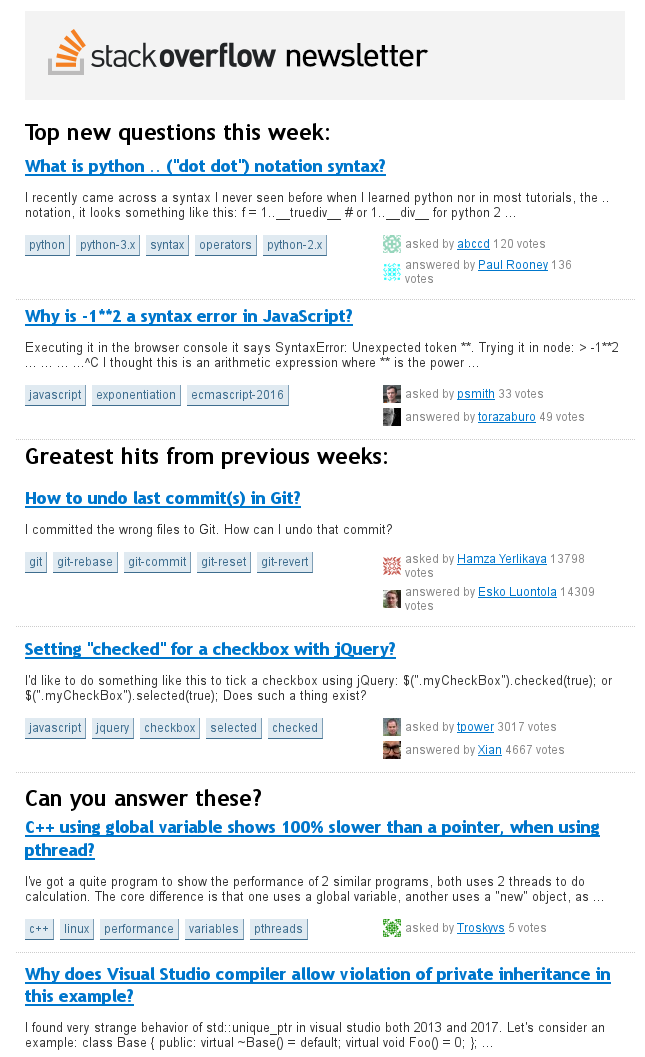
\includegraphics[scale=0.4]{so-newsletter}
\caption{Informačný bulletin komunity Stack Overflow, 25. apríl 2017.\label{fig:so-newsletter}}\end{center}
\end{figure}

\subsection{Informačný bulletin portálu Quora}

Quora\footnote{\url{https://quora.com}} je CQA systém, ktorý nie je zameraný na konkrétnu oblasť záujmu, ale obsahuje
otázky z rôznych tém. Quora ponúka svojim používateľom týždenný informačný bulletin (\emph{Quora Weekly Digest}),
ktorý obsahuje desať najzaujímavejšich otázok za posledný týždeň a zoznam ľudí, ktorých používateľ potenciálne pozná.

Zoznam najzaujímavejších otázok pozostáva z editormi manuálne vybraného obsahu a algoritmicky vybraného obsahu,
ktorý je personalizovaný pre každého používateľa zvlášť (Obr.~\ref{fig:quora-newsletter}).

\begin{figure}[H]\begin{center}
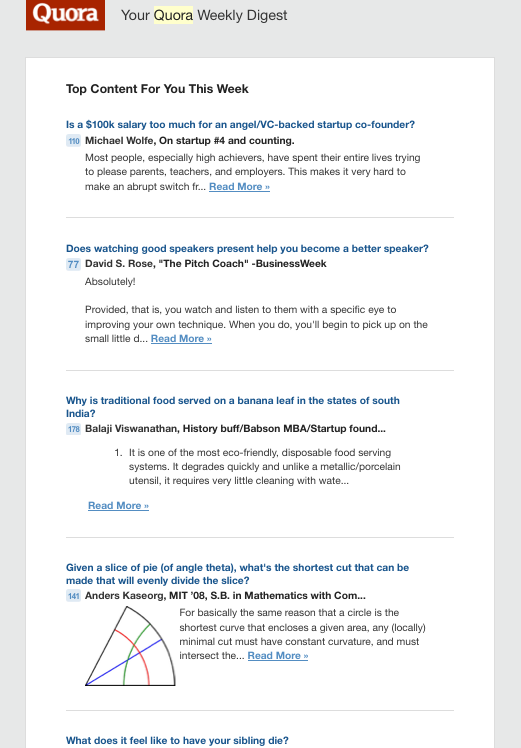
\includegraphics[scale=0.5]{quora-newsletter}
\caption{Informačný bulletin portálu Quora. Prevzaté 30.4.2017, \url{http://www.businessinsider.com/quora-emails-2012-8}
\label{fig:quora-newsletter}}\end{center}
\end{figure}

\subsection{CQA systémy bez informačných bulletinov}

Viaceré populárne CQA systémy svojim používateľom vôbec neponúkajú možnosť odoberať informačný bulletin. Medzi takéto
systémy patrí napr. portál \emph{Yahoo! Answers}\footnote{\url{https://answers.yahoo.com}}, ktorý je určený na pokladanie
otázok z akejkoľvek oblasti záujmu. Rovnako informačný newsletter neponúka ani ďalší všeobecne zameraný CQA systém --
\emph{Wiki Answers}\footnote{\url{https://answers.com}}. CQA systém zameraný na podporu výučby
\emph{Askalot}\footnote{\url{http://askalot.fiit.stuba.sk}} tiež v súčasnosti neponúka informačný newsletter,
iba možnosť notifikácie používateľa prostredníctvom e-mailu o aktivite súvisiacej s jeho obsahom v rámci systému.

%%%%%%%%%%%%%%%%%%%%%%%%%%%%%%%%%%%%%%%%%%%%%%%%%%%%%%%%%%%%%%%%%%%%%%%%%%%%%%%%%%%%%%%%%%%%%%%%%%%%%%%%%%%%%%%%%%%%%%%%


\newpage
\chapter{CQA systémy}

    - Co to je
    - Cim sa lisia od inych user-generated content sites
    - Rozdelenie CQA systemov - Yahoo Answers-type vs SO-type



%%%%%%%%%%%%%%%%%%%%%%%%%%%%%%%%%%%%%%%%%%%%%%%%%%%%%%%%%%%%%%%%%%%%%%%%%%%%%%%%%%%%%%%%%%%%%%%%%%%%%%%%%%%%%%%%%%%%%%%%


\chapter{Odporúčanie}

- Odporucacie systemy celkovo - o co ide (len kratko)
    - Content-based filtering
    - Collaborative filtering
- Odporucanie v CQA systemoch
- Question Routing, Question recommendation, retrieval... definitions...
- Challenges:
    - Cold start
    - Filter bubble



%%%%%%%%%%%%%%%%%%%%%%%%%%%%%%%%%%%%%%%%%%%%%%%%%%%%%%%%%%%%%%%%%%%%%%%%%%%%%%%%%%%%%%%%%%%%%%%%%%%%%%%%%%%%%%%%%%%%%%%%


\chapter{Diverzifikácia a aktuálnosť}

- Diverzifikacia v odporucacich systemoch -> riesenie filter bubble
- Dopad aktualnosti na uspesnost odporucania
- D and A v CQA
